\chapter{Prelude to the specification} \label{chap:informalSpec}

%%%TEST


%{\em *** Version: \today~ ***}

%reorganizing Chapter 5

\bc
Introduction

Proxima is levels with layers in between.
Here we specify the types of the levels, and what functions between them.

The defs hold for all layers and levels, although some special cases.

Renderer is implemented as tree, but
\ec




\bc

?? mention that in the process of refinement, only the last step makes sense? Direct/indirect edit ops etc. from previous chapters is not made here, and breaks invariants. Will (hopefully) be fixed in next chapter.


Duplications somewhere else? Only in evaluator.
mapping toc, two arrows, one to each group
be clear on when mapping is required. Only if lower has ls. back only if partial pres?



TODO
check super & subscripts in figures and text: h/high h,intr or h_intr, etc.

SOMEWHERE: mappings important for extra state, but also for editing on several levels. (is this really true?)

MAPPING INFO INCONSISTENCY: figure out how to express that two cycles are needed to restore it.
                                                  %is probably related to edit ops starting at higher level
ALSO ALL IS ON TREES, for other things, eg, sum of leaves, it does not work, do it yourself
EXTRA STATE, also tree ordering? precedence op tree -> non ordered op tree?
SOMEWHERE, explain why this is all necessary, refer to Editing Chapter


***EXTRA STATE is based on invariant mapping, however, implemented mapping is from level to level
***EXTRA STATE is only possible when inc. because lev, cannot be derived, or maybe only store extra?

** SOMEWHERE. pres is typically just for viewing: no big problem when destroyed
** intr is more essential. bigger problem when destroyed.
** guarantee no loss, so only limited edit func. on toc.

interpretation is bit strange as edit ops can be on higher level
* could this also be the case with presentation?


!what about sheets? 

SOMEWHERE: FOCUS more formally (if included then add forward refs to edit model chapter)


IMPL: mapping downward, how to store in doc? Now datatype changes when pres is modified

\ec


%* explain edit steps? Before fitting it all together, we first build one layer


% TODO: check if presentation mapping and interpretation mapping is used consistently.


\bc
In the layered architecture of Proxima (see Chapter~\ref{chap:proxArch}), each layer maintains an invariant between adjacent levels. When either the higher or the lower level is changed, the other adjacent level is updated appropriately. The process of updating the levels is largely symmetrical for both directions.

This chapter discusses the invariant that is maintained between adjacent levels from the perspective of a single layer. Furthermore, it specifies the additional information necessary for computing the updates that restore the invariants. The invariants given in this chapter hold for any layer in the Proxima system, although some layers are simpler than the generic layer presented here.

\ec

In this chapter, we informally introduce several concepts that play a role in the specification of a layered editor, to be given in Chapter~\ref{chap:formalSpec}. The discussion in this chapter also recapitulates some issues already mentioned in Chapter~\ref{chap:proxArch}. Although many examples come from the Proxima editor, the concepts are general and apply to any layered structure editor.

Section~\ref{sect:editProces} introduces the presentation invariant that is to be maintained by an editor and sketches the different steps of the editing process. In Section~\ref{sect:extraState} we explore the concept of extra state for presentation mappings between tree structures, and sketch a method for handling such extra state. Finally, Section~\ref{sect:informalDuplicates} discusses how to handle edit operations on presentations that contain duplicate information.


% based on a mapping between levels
% add sheets, add extra and add incrementality

%\note{somewhere: Stress that mappings are not needed when for subtrees for which the lower level is not editable}
%\note{somewhere: Stress that it's only an architecture. Safety, impl. etc is left to layer. Future research (Pierce?)}
%rather than safe toy, complete arch for many ed's Safety and patterns need to be researched

\bc
Where say that mapping back is only when we need automatic editing: is it only important for duplicates? It seems to be important for 2:1 presentations as well.  In some complicated cases, the mapping back cannot be spec'd if mapping back is does not work, it means that lower edit cannot be handled, and is forbidden. However, we always have the higher-level edit left.
\ec



%																
%																
%																
\section{The editing process}\label{sect:editProces}

% during editing one of the levels is changed, other changes along. in this section first give updates for entire editor
%, then refine it for layers


An editor maintains a presentation relation between a document and its presentation. We denote the document by 
$level\H \tp Level\H$, and the presentation by $level\L \tp Level\L$. The relation between the two is
$\Present \tp \Level\L \rel \Level\H$.  The level order in the relation type is such that the notation $l~Present~h$ looks similar to the notation for a presentation mapping represented by a function: $l = \present~h$. 

%$R \tp Range \rel Domain$ versus $f \tp Domain \to Range$

The invariant, maintained by the editor is that the lower level is a valid presentation of the higher level:

\begin{math}
\text{\bf Presentation invariant:~~~} \level\L~\Present~\level\H\\
\end{math}

\finallongpage
The precondition of an edit step is that the presentation invariant holds. The user then modifies the presentation (giving $\level'\L$), and most likely breaks the invariant. In order to restore the invariant, the editor updates the document level by interpreting the modified presentation, which yields $\level''\H$. However, because the user-updated lower level is often not a completely valid presentation, the document update alone may not yet restore the presentation invariant. For example, a program fragment may have been entered without proper syntax coloring, or a chapter title may have been modified in the chapter itself but not in the table of contents. In order to guarantee the restoration of the presentation invariant, the updated document is presented again ($\level''\L$).

Figure~\ref{singleLayerEdit} schematically shows the editing process for one edit step.  The final higher-level value is called $level''\H$ rather than $level'\H$ to enable a consistent notation for final values. Furthermore, in the multi-layered editor, introduced in the next section, $level'\H$ will denote an intermediate value for the higher level.

The final values $level''\H$ and $level''\L$ satisfy the presentation invariant and serve as initial values for the next edit step. In the rest of this chapter, as well as in the next, we use this notation for the values of the data levels in the different stages of an edit step.

\begin{figure}[h]
  \hfill
  \begin{minipage}[b]{.45\textwidth}
    \begin{center}   
      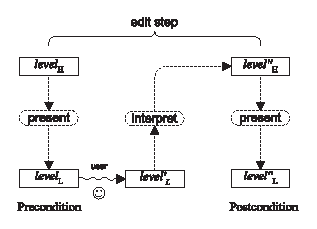
\epsfig{file=pics/eps/LayerSimple.eps, height=1.4in} %width = 60mm}
      \caption{A single edit step.} \label{singleLayerEdit}  % visio: Layer.vsd
    \end{center}
  \end{minipage}
  \hfill
  \begin{minipage}[b]{.45\textwidth}
    \begin{center}  
      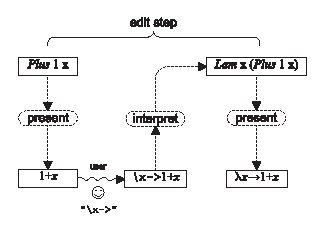
\epsfig{file=pics/eps/LayerExample.eps, height=1.4in} %width = 60mm}
      \caption{A concrete example.} \label{singleLayerEditExample} % visio: Layer.vsd
    \end{center}
  \end{minipage}
  \hfill
\end{figure}

%
%\begin{figure}
%\xpr{
%level\H 		&   			&		 & 			& level''\H\\
%~~~\downarrow &   		&		&~\nearrow~&~~~\downarrow \\
%level\L 		&~\leadsto~ & level'\L 	& 			& level''\L\\
%}
%\caption{Single edit step schematically.(draft)} \label{singleLayerEdit}
%\end{figure}

%\begin{figure}
%\xpr{
%Sum~1~x 		&   			&		 & 			& Lam~x~(Sum~1~x)\\
%~~~\downarrow &   		&		&~\nearrow~&~~~\downarrow \\
%1+x 		&~\leadsto~ & {\tt \backslash x~->~} 1 + x 	& 			& \lambda~x~\to~1+x\\
%}
%\caption{Single edit step example.(draft)} \label{singleLayerEditExample}
%\end{figure}

Figure~\ref{singleLayerEditExample} shows the values of the higher and lower levels for an actual example. The document is an expression that is presented using an italic style for identifiers and mathematical symbols for operators. The presentation of a sum in modified by entering the text "\verb|\x->|" at the beginning. After the document update, the presentation invariant clearly does not hold. It is restored by re-presenting the document, and thus changing "\verb|\x->|$1+x$" to "$\lambda\hspace{0.5pt} x \to 1+x$".


Instead of updating the lower level (presentation-oriented editing), a user may also perform an direct update on the higher level (document-oriented editing). However, we do not consider document-oriented editing in much detail, because after a document update the presentation invariant can be restored by simply re-presenting the updated document.


\bc
$\Present$ and $\Interpret$ are not actual functions that can be evaluated, but abstract concepts used to express a property of two levels. The functions are used to specify the behavior of a layer.
Strictly speaking, $\Present$ and $\Interpret$ are not even functions but relations, since a higher level may have several correct presentations, and a lower level may have several correct interpretations. However, this occurs only if a level has extra state, as will be explained in Section~\ref{sect:extraState}. \ec

\bc Because we only look at one layer in this chapter (ie. the layer between $\Level_{H}$ and $\Level_{L}$), we need two more functions to refer to the behavior of the layers below this layer, as well as the layers above. For lower layers, the function 
$\Edit :: \Level_{L} \rightarrow \Level_{L}$ denotes an update on $\Level_{L}$ by the lower layers. For representing updates on the higher level, we use 
$\Transform :: \Level_{H} \rightarrow \Level_{H}$. In the next chapter, when layers are connected, $\Edit$ and $\Transform$ become superfluous.\ec


\head{A layered editor}

% why layers?
In order to describe the layered architecture of Proxima (see Chapter~\ref{chap:proxArch}), we refine the simple editor by splitting the presentation relation. A $Present$ relation that is split into $n$ components 
($Present_{i} \tp Level_{i} \rel \Level_{i-1}$) gives rise to $n+1$ data levels ($Level_{0 \dots n}$). Lower levels get higher indices, with $Level_{0}$ being the document level and $Level_{n}$ the presentation level. 

From the perspective of a single layer, we only need to consider a single $Present_i$ relation and two data levels $Level_{i-1}$ and $Level_{i}$. We drop the subscript of the relation and refer to the data levels as $Level\H$ and $Level\L$. Figure~\ref{layerEditProcess} shows the updates during an edit step from the perspective of a single layer. 
Instead of being updated immediately by the user, the lower level gets updated by the layer below (which is the effect  of the user updating the lowest level). At the top of the figure, the layer computes an intermediate $level'\H$, instead of directly computing $level''\H$. This $level'\H$ is processed by the layers above, yielding $level''\H$. At the document level, $level'_0$ is copied to $level''_0$. Note that there is no incrementality in the model: level values are passed up and down, but not to the right. 
% \nonote{mention doc edit on intermediate levels?}


% can we express when this happens with a condition? pres .. /= pres .. oid?

A simple example shows the need for the intermediate $level'\H$. Consider a document that consists of a list of numbers, which is mapped onto an enriched document that contains the list together with its sum. The presentation is a textual presentation of both the list and the sum. Suppose that the list is edited at the presentation level. At the presentation layer, the updated presentation is parsed, yielding an intermediate enriched document value $level'\H$, which is the new list with the old sum. This intermediate value is then interpreted and presented by the evaluation layer above, yielding the final $level''\H$, which is the updated list with a correct sum.

\begin{figure}
\begin{small}
\begin{center}
\begin{center}
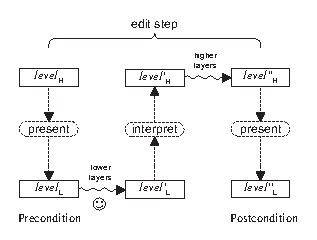
\epsfig{file=pics/eps/LayerSingle.eps, height=1.4in}  % visio: Layer.vsd
\end{center}\caption{An edit step at one layer.}\label{layerEditProcess} 
\end{center}
\end{small}
\end{figure}
% original layered picture was not very clear.

% why two:
\bc
We use two invariants instead of one, to make it possible to describe the intermediate state in which changes have not been fully propagated upwards and been taken into full account. Consider an editor in which an enriched document node for a product expression (\verb|Product (Int 1) (Int 2)|) is presented as a list of presentation level tokens, colored according to the syntax. The integer values are presented in black, and the operator in green. If we denote the colors between braces, the presentation is \verb|["1" {black}, "*" {green}, "2" {black}]|. Because the presentation level is a correct presentation of the document level, the presentation invariant is satisfied. But now consider a list of tokens typed by the user, which do not have the correct coloring: \verb|["1" {black}, "*" {black}, "2" {black}]|. If we use a single invariant, then expressing that \verb|Product (Int 1) (Int 2)| is an appropriate interpretation of the uncolored tokens list, also implies that the uncolored tokens are a correct presentation of the product expression. It is no longer possible to express that the colored presentation is a correct presentation of the product, whereas the uncolored presentation is not. \note{are we saying that with one invariant, pres is inverse of intr?} \ec



\bc

OTHER EXAMPLE?: Apart from the syntax coloring example, the problem also arises when for example a textual arrow 
\verb|"->"| is presented as a $\rightarrow$. 

Vice versa? Fix by remembering extra?
 layer shortcutting can now be expressed by only letting the lower pres invariants hold

 -explain that in incremental, present and interpret cannot be used instead of Present and Interpret
 -how does this relate to inc with diff etc. maybe that can be expressed nicely with Present
 (or even present, then Present will be superfluous.)

* does   intr.pres = id hold for a layer? pres.intr never needs to hold due to syntax coloring, normalization etc., but also because Chess board is not a presentation of ChessBoard   
* intr.pres = id? then each pres has unique doc. Is this true? Can't doc variants be presented as same thing?
   present( interpret uncolored ) = colored, so present.interpret /= id
   interpret ( present ) = id? if so, what if two docs are presented on the same pres?
 it seems true, interpret.present cycles should not alter the doc. In case of ambiguity, the system should
 take care of conservative behavior. On an edit, the doc may change, but that's not a (interpret.present) cycle

****** When this is figured out, update sheet paragraph
\ec




%																
%																
%																
\section{Extra state} \label{sect:extraState}

%SOMEWHERE: when es is hard. If no parent with a presentation is parent then 
% tricky. Hence invisible nodes with extra state may lose it during editing.


As we saw in Section~\ref{sect:editingExtraState}, a lower level may contain information that cannot be computed by presenting its adjacent higher level. Similarly, a higher level may contain information that cannot be computed by interpreting the lower level. The information in a level that cannot be computed by presenting, or interpreting an adjacent level, is referred to as {\em extra state}. In this section, we give an informal description of extra state, as well as a number of examples. Section~\ref{sect:singleExtra} presents a formal specification.

Generally speaking, {\em presentation extra state} is information that influences the way in which the higher level is viewed without being part of the higher level. An example of this is found in a tree-browser presentation (see Section~\ref{sect:treeBrowser}). The information whether a node in the tree is expanded or collapsed is not part of the document. Therefore, this expansion state is part of the presentation extra state.

{\em Interpretation extra state}, on the other hand, consists of the parts of the higher level that are not shown in the presentation. Again, the tree browser provides an example, since it shows the structure of the document while leaving out the content. The content that is left out is part of the interpretation extra state.

Because the presentation or interpretation does not specify the value of the extra state in the resulting level, extra state is reused, if possible, from the previous value of the level. A general method for reusing extra state is difficult, if not impossible, to give. Therefore, in this section, we consider a special case of extra state, for which we sketch a method for reuse. We only consider extra state that is associated with a specific parent node in the tree. Whether or not the extra state can be reused depends on whether or not its parent node can be tracked down in the updated level. This form of extra state is sufficient for specifying the use cases presented in Section~\ref{sect:usecases}. Chapter~\ref{chap:formalSpec} contains a more formal specification of extra state.

%\note{explain what this kind } First, we take a closer look at the presentation, followed by an informal definition of extra state. %Finally, we sketch how it can be reused.


%\bl   % coming from formal chapter
%\o move these to first half (or previous chapter)
%\o Examples Pres: tree browser expansion state, table view sorting, file manager details/icons (positions), layout.
%\o Intr: Structure view.
%\el

%In this section, we discuss the two give an informal definition of extra state and also sketch how extra state can be reused.
%refine the definitions of the data levels in order to give a more precise definition of this extra state. Furthermore, we specify %what information needs to be kept track of in order to handle extra state.


%This section explains : welke info. wanneer gaat het mis. 



%																
\subsection{The presentation mapping}\label{mappingsInLayer}

% mapping is relation levelH levelL but each two levels express a mapping between nodes.

In order to specify when a node is extra state, we first take a closer look at the presentation relation. In this section, we assume that both $Level\H$ and $Level\L$ are tree structures. Furthermore, we assume that $Present$ not only relates a higher level to a lower level, but that it also establishes a relation between the nodes on these levels. If, for example, a document containing an if expression is mapped onto a presentation that contains the three tokens ``\p{if}'', ``\p{then}'', and ``\p{else}'', then this establishes a relation between the \p{If} node in the document, and the three token nodes in the presentation.
Thus, for any two levels $Level\H$ and $Level\L$ between which the presentation invariant holds, we also have a relation between the nodes of these two levels.
\bc Hence, we have two relations; a relation between the upper and lower trees, and a relation between the nodes of these trees. An example shows what we mean by this. \ec

Figure~\ref{nodeMapping} shows two levels for which the presentation invariant holds. In addition, the figure shows the relation between the nodes of both levels, using dotted arrows. To reduce the number of arrows in the figure, the lower-level nodes are grouped. An arrow between two nodes only relates the nodes and not the subtrees rooted at these nodes. % \nonote{why not?}

We assume that the relation between nodes is a $1:n$ relation, which implies that the presentation of a higher-level node may consist of several lower-level nodes, but each lower-level node is in the presentation of at most one higher-level node. This restriction concerns only the node mapping; the $Present$ relation itself between two levels is $n:m$. 

The choice for $1:n$ relations follows naturally from the compositional way in which a presentation relation is usually specified: by specifying a presentation rule for each higher-level node. No practical examples have been found that suggest $n:m$ relations are needed.
%\nonote{maybe just say $n:m$ here and mention later that in Proxima we have $1:n$?}

The $1:n$ restriction is only for dealing with extra state. It is still possible to have a lower-level node depend on several higher-level nodes, but when dealing with extra state, each lower-level node is assumed to be the presentation of at most one higher-level node.


% (mention fold/ag?) 
%What about focus?, is that the reason?
%Parser makes it hard to do n:m reuse. For eval layer might be possible already.

\begin{figure}
\begin{center}
\begin{center}
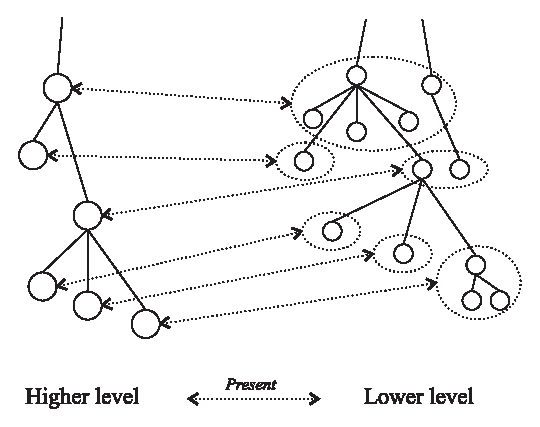
\epsfig{file=pics/eps/mapping.eps, width=2in}
\end{center}
\caption{A mapping between the nodes of two levels.}\label{nodeMapping} 
\end{center}
\end{figure}



\begin{figure}
\begin{center}
\begin{center}
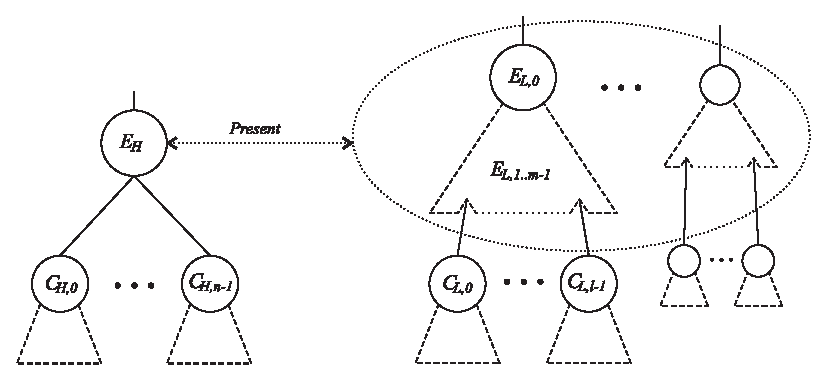
\epsfig{file=pics/eps/presentationEh.eps, width=80mm}
%\begin{verbatim}
%                  ..
%                    \
%..                   EL0
%  \                 ELEL.
%   EH       ->     EL..EL.
%  / \             EL....EL. 
% C...C           EL......EL.
%                EL/\EL.EL/\EL.
%                 /__\   /__\
%                    
%\end{verbatim}
\end{center}
\caption{The presentation of node $E_H$.}\label{nodePresentation} 
\end{center}
\end{figure}

Thus, besides relating a set of higher-level values to a set of lower-level values, $\Present$ also relates each node of the higher level to zero or more lower-level nodes. Figure~\ref{nodePresentation} schematically shows the presentation of a node ($E_H$) in the higher level. $E_H$ has $n$ children ($C_{H,0\dots n-1}$). The presentation of $E_H$ is a number of trees (although usually just one) that may consist of several nodes. In the figure, the first tree is shown in more detail. It consists of $m$ nodes ($E_{L,0\dots m-1}$) and is rooted at $E_{L,0}$. 

The $C_{L,0}$, \dots, $C_{L,l-1}$ subtrees in the lower-level tree are not part of the presentation of $E_H$. Typically, these are the presentations of the children of $E_H$, but in general they can be (part of) the presentation of any node in the higher level. 

\begin{figure}
\begin{center}
\begin{center}
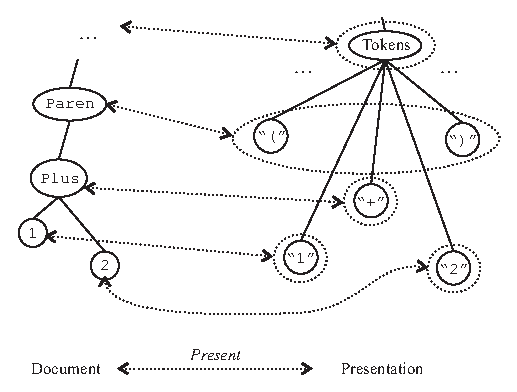
\epsfig{file=pics/eps/presentParenSum.eps}
%
%  ( )       Tk   ( 1+2 )
%   +      Tk ...
%  1 2       .....  
%
\end{center}
\caption{The presentation of a parenthesized sum.}\label{presentExample} 
\end{center}
\end{figure}

%removed story about whitespace extra state
Figure~\ref{presentExample} provides a more concrete example of a presentation, taken from a source editor (see Section~\ref{sect:sourceeditor}). A parenthesized sum in the document is presented as a list of tokens, which are represented by strings.  The figure shows only part of the document and its presentation. To the editing user, the expression will appear as "{\tt (1+2)}". The example is somewhat simplified, because it does not contain whitespace. Whitespace is part of the presentation extra state, which is discussed in following subsection.

\bc  why is this one commented?
In the example, the resulting presentation is a single tree, but this is not always the case. For example, the evaluation layer in a word processor (see Section~\ref{sect:wordprocessor}), maps each chapter onto an entry in the table of contents, as well as onto the presentation of the chapter itself. Hence, the presentation (in this case the evaluation) of a chapter consists of two separate enriched document trees.
\ec






%																
\subsection{Extra-state nodes}

In Figures~\ref{nodeMapping} and~\ref{presentExample}, each node is connected to a node in the adjacent level, either by a direct arrow, or by being inside an ellipse that is connected by an arrow. However, it is possible that a node does not have an arrow connecting it to a node in the adjacent level. Such nodes are not determined by the presentation relation, and hence are part of the extra state of the level.

%** mention that es elt must be associated to parent.

Extra state may occur on the higher level as well as on the lower level. On presentation, a lower level is computed from a higher level, which means that the extra state in the lower level needs to be dealt with. Hence, lower-level extra state is referred to as {\em presentation extra state}. Similarly, on interpretation of a level, we only need to deal with the higher-level extra state, which is referred to as {\em interpretation extra state}. In fact, if we consider not just one layer, both kinds of extra state may exist on a single level. This is explained in Section~\ref{sect:oneLevelDoubleES}.

\bc
during is not okay+ levels benoemen, want er wordt vaak heen en weer gesprongen.

% One layer: two kinds of extra
Since a presentation of a node may consist of zero or more nodes, and an interpretation consists of at most one, it is possible that a node is not mapped onto any nodes in the target level. In that case, the target level simply does not contain the information needed to compute the node**iets specifieker**, and hence it ** what ** is part of the former level's extra state. Because whether or not a node is extra state depends on which mapping we consider, we distinguish two kinds of extra state: presentation extra state and interpretation extra state. The {\em presentation extra state} consists of nodes that during presentation cannot be computed from the higher level (the shaded nodes at the top level of Figure~\ref{layerExtraState}), and the {\em interpretation extra state} consists of nodes that during interpretation cannot be computed from the lower level (the shaded nodes at the bottom layer of the figure).
\ec


% example pres extra
Figure~\ref{layerExtraState} shows two examples of extra state, one in the lower level and one in the higher level. On the left-hand side, a document node is presented as a token. The shaded whitespace node (0,1) (denoting the line-breaks and spaces before the token) is not specified by the presentation mapping, and hence part of the lower level presentation extra state. On presentation, tokens are reused, causing the whitespace information to stay the same. In order to do this, we need to know exactly on which presentation nodes a document node was mapped when it was previously presented. In case a token has no previous whitespace (e.g.\ because it is the presentation of a newly inserted document part) a default value is used.

\begin{figure}
\begin{center}
\begin{center}
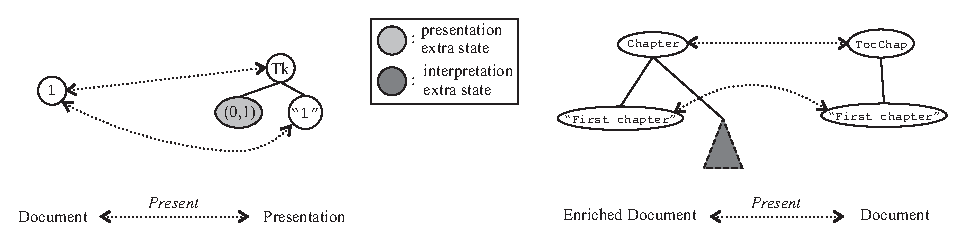
\epsfig{file=pics/eps/presIntrESExamples.eps, width=125mm}
\end{center}
\caption{Two examples of extra state.} \label{layerExtraState} 
\end{center}
\end{figure}

% example intr extra

The right-hand side of Figure~\ref{layerExtraState} shows an example of interpretation extra state: a word processor with an editable table of contents. A document chapter is presented only partially, since the content of the chapter is left out.

For simplicity, we assume that the enriched document only contains the table of contents and not the chapters themselves. Thus, we only have to consider the extra state here and not the duplication (titles that appear in the table of contents as well as in the chapters). Section~\ref{sect:informalDuplicates} discusses how to handle duplications in general, and the same method can be used for the table of contents.

On interpretation, the table of contents is mapped back onto a complete document, which includes the shaded content parts that are not in the enriched document. The title of a chapter comes from the enriched document, whereas its content is reused from the previous document.



\bc
An important point to note is that extra state with regard to a certain mapping is extra state for the {\em result} type of the mapping. Hence, presentation extra state for a presentation mapping between $\Level_{H}$ and $\Level_{L}$ is in $\Level_{L}$. Vice versa, interpretation extra state is in $\Level_{H}$.
\ec

\bc Although the term presentation extra state of $\Level_i$ may suggest that this concerns state that is used during the presentation of $\Level_i$, this is not the case. The extra state of $\Level_i$ refers to the extra state with regard to the presentation of the level above ($\Level_{i-1}$) on level $\Level_i$. The only extra state that is involved in the presentation of $\Level_i$ is that of its lower neighbor: $\Level_{i+1}$
\ec


%																
\subsection{Each intermediate level has two kinds of extra state} \label{sect:oneLevelDoubleES}

% One level: two kinds of extra
Figure~\ref{layerExtraState} only shows one layer, but since each data level except the document and the rendering is in between two layers, each level between the document and the rendering may have both presentation and interpretation extra state. 

Figure~\ref{levelExtraState} shows a data level between two layers. At the middle level, a shaded left or right half denotes that a node is extra state. Nodes with a shaded left half are presentation extra state for the higher layer, and nodes with a shaded right half are interpretation extra state for the lower layer. Extra state in one direction is independent of extra state in the other direction, hence a node in the figure can have zero, one, or two shaded halves.

\begin{figure}
\begin{center}
\begin{center}
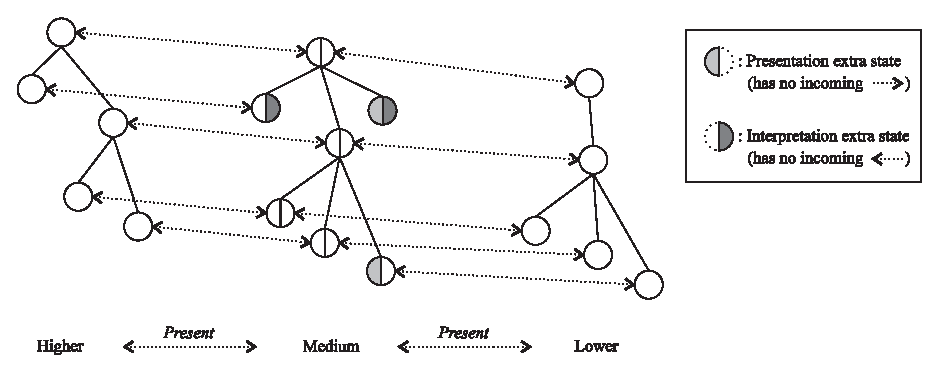
\epsfig{file=pics/eps/3levelES.eps, width=125mm}
\end{center}
\caption{Presentation and interpretation extra state in one level.}\label{levelExtraState} 
\end{center}
\end{figure}

% example one level independence of es
The whitespace extra state in tokens shows that extra state in one direction is independent of extra state in the other direction. Whitespace is presentation extra state of the presentation level, since it cannot be computed when presenting the enriched document. On the other hand, when scanning, whitespace in tokens is computed from strings and line breaks in the layout level. Hence, whitespace is not interpretation extra state of the presentation level.

%\note{also example of one level with both kinds of extra state? Will be somewhat contrived}


\bc
When the scanner layer interprets the layout level, spaces and row transitions between a token's string and the preceding token's string are encoded as whitespace information in the token. Since it can be computed during interpretation, the whitespace is not part of the interpretation extra state. On the other hand, when the enriched document is presented on tokens in the presentation level, the whitespace information cannot be computed, and hence it is part of the presentation extra state of the presentation level.
\ec

\subsection{Reusing extra state}

When a new value for a level is computed on presentation, or interpretation, the values for its Extra-state nodes are taken from the previous value of that level. 

%\note{mention that we only need to keep track of roots?}
In order to reuse nodes, a layer needs to keep track of additional information regarding the presentation mapping. For each higher-level node, the layer must keep references to the lower-level nodes of its presentation, and for each lower-level node there must be  a reference to the higher-level node whose presentation it is part of. These references corresponds to the dotted arrows between nodes in the figures of this section.

We sketch the process of reusing for the presentation direction. For interpretation, the process is analogous.

We assume that the update on the higher level is incremental; except for the parts that have been edited, the updated level is equal to its previous value.  On presentation of a higher-level node, the lower-level nodes of its previous presentation are used to construct its new presentation, if possible. If the higher-level node is new, the presentation will consist of new lower-level nodes. Furthermore, also in case the node was changed in such a way that its previous lower-level nodes cannot be reused, new lower-level nodes are used.

The resulting lower level is not a completely new value, but an incrementally updated version of the previous value. Only those parts of the presentation that correspond to a changed part of the higher level are changed. 

When a lower-level node is reused, also its Extra-state children are reused.  For nodes that are no longer present in the presentation, Extra-state children are lost. Extra-state children for new lower-level nodes are set to a default value. Thus, if an entry is added to a table of contents in the (presentation of the) enriched document of a word processor, an empty chapter (or section) is added to the document. Similarly, if a document-oriented edit operation in a source editor adds a new structure to the document, its presentation gets a default layout.


\subsection{Safety of extra state}

The mechanism of reusing extra state based on its parent nodes is not infallible. Several situations can cause the loss of extra state, both in the presentation as in the interpretation direction. We present two situations here.

Firstly, if the presentation of a node depends not only on the node itself, but also on nodes elsewhere in the tree, then the presentation may change, even if the node itself remains unchanged. In that case, it is possible that the lower-level nodes of the previous presentation cannot be used for the new presentation.

For interpretation extra state, updates elsewhere in the tree can be  even more dangerous. When a presentation is computed by a parser, updates on the presentation before a certain token may greatly influence how the token is parsed. Hence, extra state in a presentation that allows full text editing is vulnerable. 

%\note{Mention imprecise edit? When interpreted presentation is much different from final presentation, es reuse may be tricky 
%(e.g.\ after entering "{\tt ->}", final presentation is "$\rarr$"?)}

Secondly, if a node is transformed, it may make sense to reuse its extra state in the result of the transformation. For example, when in an expression editor, a sum node at document level is transformed to a product node, it makes sense to reuse its whitespace extra state. However, if the transformation is performed by simply removing the old sum and inserting a fresh product node, then the extra state is lost. In such a case, an editor designer may specify for a transformations that source nodes are reused in the result, thereby also reusing their extra state. 

More research is necessary to establish clearly in what situations extra state is vulnerable, and also how reusing it can be maximized. Although in general it cannot be guaranteed that extra state is always recoverable, this does not necessarily pose a problem. Because presentation extra state generally consists of non-essential information, it is not a big problem that in some rare cases, it is reset to a default value.

Interpretation extra state, on the other hand, may represent essential information, but by restricting the edit behavior on presentations that have interpretation extra state, an editor designer can protect it from accidentally getting lost. For example, the edit behavior on a table of contents can be restricted to updates on titles, and insertion and deletion of entire entries. For these edit operations, the reuse of extra state does not fail. Furthermore, a warning may be issued when document extra state is about to get lost, for example when a user deletes a table of contents entry.

\subsection{Conclusions}

The method of handling extra state, presented in this section, applies only to extra state that is clearly associated with a certain parent node. The method works for specifying the whitespace extra state for token presentations as well as interpretation extra state for editing partial presentations. However, the method of reusing is only sketched, and the exact way in which to reuse extra state is left to the editor designer.

Extra state is vulnerable, and it is easy to create situations in which reusing it is impossible, for example by allowing full text editing in a presentation that hides a large part of the document. However, the point is that the model allows those instances of extra state that are useful and for which a clear method of reuse can be established.

Extra state in one layer also has consequences for the other layers in the editor. In order to reuse presentation extra state, the higher-level nodes must have a reference to their previous presentation. Hence, the layer above must reuse the higher-level nodes when computing the higher level (by presenting the level above it). The references to the lower level can be considered presentation extra state of the higher level. The same thing holds for interpretation extra state: references from the lower level to the higher level can be considered interpretation extra state of the lower level.

Besides extra state that is attached to a certain parent node, other forms of extra state exist. For example, when a list in the document has a fixed order, but is allowed to be reordered by the user in the presentation, the order can be seen as either presentation or interpretation extra state.


Since extra state arises whenever a presentation or interpretation mapping has no unambiguous inverse, many other kinds of extra state exist. Further research is required not only to establish more precisely how to deal with extra state attached to a certain parent, but also to establish other kinds of extra state, as well as methods of handling it. Finally, it would be desirable to have automatic handling of extra state for certain kinds of presentations (or interpretations).



% Partial ES: present (4) = "Int"
\bc
Even if a node $E_H$ is mapped onto one or more nodes in the lower level, it can still be part of the extra state if these lower-level nodes do not constitute enough information to compute $E_H$. Consider for example a presentation of a Haskell source, in which al integers are presented with the string \verb|{Int}|. The integer nodes do have a presentation, but since it does not contain enough information for the backward mapping, the integer nodes are in interpretation extra state. \note {Is this also the case for focus?} 
%\note{Don't know much about this kind of ES yet}
\ec
%%%


%%% stuff on 1:n vs  n:m
\bc
A consequence of the difference between the presentation and the interpretation mappings is that even when a lower-level node depends on several higher-level nodes, only one is responsible for its presentation. For example, when a node \verb|Word Color String|, representing a colored string, is presented as a string in the specified color. Now the string in the presentation is presentation of \verb|Color| as well as of \verb|String|. However, only one of the two can be the interpretation of the . In order to edit the color
\ec

%IntExp int problem: ignore elts with no pres and build fresh when interpreting? 










%																
%																
%																
\section{Duplicates in the presentation} \label{sect:informalDuplicates}

%\note{mention duplicates in interpretation?}
%* not just because multiple trees: nodes may depend on several trees. without duplication.

Duplication occurs when a higher-level structure is presented on more than one lower-level structure. An example of duplication is a chapter title that appears both in the derived table of contents as well as in the document. But also multiple windows with (possibly different) presentations of the same part of the document give rise to duplications. 

The problem with duplicate values is that if only one of the duplicates is edited, a conflict may arise during interpretation, and the editor needs to choose which value to use for computing the higher level. As mentioned already in Section~\ref{sect:reducer}, we tackle the problem by giving priority to the changed duplicate. In case both duplicates have been edited and yield different higher-level results, the editor can either prohibit the edit operation, or make a default choice for one of the duplicates.

It is hard to give a precise definition of duplication of information without making additional assumptions on the presentation mappings and level types. Moreover, even if part of a presentation is a duplicate, the editor designer may prefer not to regard it as such. The "\verb|(|" and "\verb|)|" tokens in Figure~\ref{presentExample} are both in the presentation of the \verb|Paren| node, but it is not immediately obvious to consider these tokens duplicates. Consider for example a presentation \verb|(1+2)*(3+4)| in which the middle two parentheses are deleted. If parentheses are regarded as duplicates, the result will be the deletion of both pairs of parentheses, yielding \verb|1+2*3+4|. However, it may be considered more natural to get the result \verb|(1+2*3+4)|.


\bc
If a higher-level node The presentation of a higher-level node may consist of several lower-level nodes, as shown in Figure~\ref{presentExample}. In this case, both the "\verb|(|" and "\verb|)|" tokens are in the presentation of the \verb|Paren| node. However, it is also possible that a higher-level node is duplicated in the presentation, in which case interpretation of the lower level may yield conflicting values for the higher-level node. An example of such a duplication is the title of a chapter that appears in the table of contents as well as in the presentation of the chapter itself. When the lower level is interpreted, several alternatives for one node may arise, and a choice has to be made.

Note that having several lower-level nodes does not automatically mean that a node is duplicated. Furthermore, the interpretation of duplicates only needs to be dealt with if the duplicate structure is edited on the lower level. If a duplicate only needs to support document-oriented editing and no presentation-oriented editing, no extra work needs to be done.
\ec

In Proxima, the only layers potentially giving rise to duplicates are the evaluation and the presentation layers. The presentation mappings for the other layers are largely predefined and do not duplicate any structures. 
\bc To avoid having to deal with duplicates when parsing, duplicating is currently only allowed at the evaluation layer. This restriction may be lifted in a future version, but for now, if a presentation contains duplicates, the evaluation sheet specifies how the involved structures are duplicated, and the reduction sheet specifies how updates on duplicate structures are handled.
\ec

\begin{figure}
\begin{center}
\begin{center}
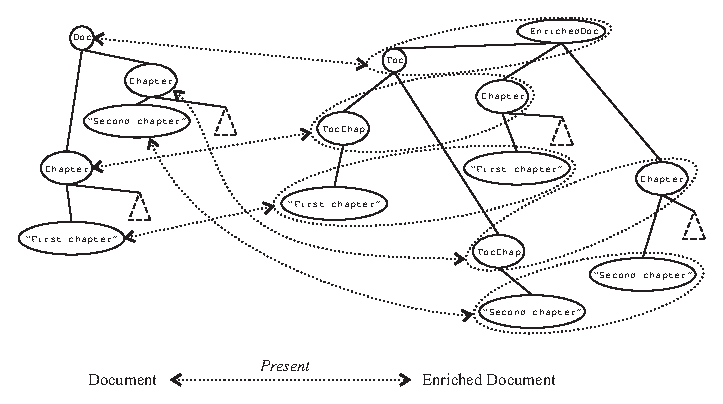
\epsfig{file=pics/eps/interpretToc.eps}
%
%  Chap              Toc
%  "first.."     TokChap      Chap
%                   "first.."     "first.." 
%
\end{center}
\caption{The presentation of a word processor document with a table of contents.}\label{duplicatesExample} 
\end{center}
\end{figure}

% example

Figure~\ref{duplicatesExample} shows an example of a duplicated structure in the form of a table of contents for a word processor. On the left-hand side of the figure is a document that contains two chapters, of which only the titles are shown. The enriched document contains both a table of contents subtree (\verb|Toc|), as well as a copy of the chapters. The table of contents subtree follows the structure of the original document, but only contains the title of each chapter rather than the chapter itself. To keep the figure simple, the table of contents only contains chapters and not sections and subsections, but in a real editor the table of contents may reflect the entire document structure. 

The evaluator maps a chapter in the document on a chapter in the enriched document, as well as on a chapter entry in the table of contents tree, in the latter case leaving out everything but the title. The presenter presents both the table of contents tree as well as the chapter tree, and does not duplicate any structures. The example also involves extra state, since a chapter is shown without its content in the table of contents. However, the extra state is orthogonal to the presence of duplicates and can be handled as sketched in Section~\ref{sect:extraState}.

When a user performs an update on the presentation, this results in an updated enriched document. Updates can be either in the table of contents, or in the chapters themselves. If the update is not in the table of contents, the document is computed from the chapters in the enriched document, while ignoring the table of contents altogether. On the other hand, if the table of contents tree is modified, the chapters in the enriched document tree are ignored on interpretation, and the document is obtained from the table of contents tree only. In this case, the chapter content is treated as interpretation extra state. 

By treating the table of contents as a partial duplicate of the chapters, it is easy to support structural updates on the table of contents, such as swapping two titles. The reuse process for extra state takes care of swapping the chapter content correspondingly. The editor designer only needs to specify what happens when a new title is inserted, or when an entry is moved to a different level (e.g.\ a section to a subsection).

%\note{mention that we need change management as well as incremental updates for this to work?}

\bc
For duplicate structures, the enriched document contains several alternatives, which may have different interpretations. In the table of contents example, the alternatives for a chapter title are the title in the table of contents and the title in the chapter. Three situations are possible. Firstly, if none of the alternatives have been edited, all interpretations are equal, and any one can be chosen. Secondly, if one alternative has been edited, the choice is in favor of the edited node. Hence, if a chapter title is edited in the table of contents, the resulting reduced document contains the updated title. Finally, if a title has been edited in the chapter as well as in the table of contents, the editor may give preference to the chapter title. In this case the edit operation may be forbidden, or either one of the values may be chosen.
%skipping eval layers becomes tricky now. but it's not mentioned here anyway
\ec

% not true, and also more implementation than specification
\bc
Specifying duplications in the evaluation and reduction sheets is not ideal, since the enriched document type now depends on whether or not the presentation contains duplicates. Hence, if a presentation contains several views on a structure, the necessary duplications for these views need to be specified in the evaluation layer. A special facility for specifying common duplicate presentations, such as tree views on a structure, in the presentation layer is desirable. A possible approach for such functionality is a special parser that can resolve duplicate conflicts during parsing. With such a parser, the entire process of handling duplicates takes place in the presentation layer, and the evaluation layer is not affected. 
%\note{parse (dirty arrangement) $\rightarrow$ dirty presentation? May be tricky as well}
\ec

%*** mention that we need change management as well as incremental updates for this to work?


\section{Conclusions}

In this section we described the editing process of a layered editor, as well as two concepts that play a role in the design of such an editor. The first concept is extra state, which may have two forms. Presentation extra state is information that cannot be computed by presenting the higher level, whereas interpretation extra state cannot be computed by interpreting the lower level. Both forms may exist independently at one level.

When the higher and lower levels are tree structures, we can identify a form of extra state consisting of nodes (or subtrees) that are clearly attached to a certain parent node in the tree. Such extra state may be reused after an edit operation by looking up the parent node in the previous value of the level (before the edit operation was applied). If this fails, a default value is used.

%\bl
%\o in general any present without inverse.  pres is tricky
%\el

The second concept that was discussed is the duplication of information in a presentation. When a presentation contains duplicates and a user edits one (or both) of these duplicates, a conflict may arise on interpretation. In Proxima, we resolve such conflicts by giving priority to the edited duplicate. In case both duplicates are edited, a default choice is made, or the edit operation is prohibited, depending on which behavior is specified by the editor designer.

%%% OLD MAPPING INFO STUFF


%Example Decl, Decl Type Exp., Tree view
%So always Info Pres and Intr. bla core extra:

\bc
% equations:      
\toHere
talk about isomorphism, instead of viewing
\fromHere
More specifically a data level ($\Level_{i}$) can be viewed in two ways, depending on the direction of the mapping function of which it is the result. When coming from the higher layer, the level can be considered as the product of a core part ($\Core_{\Pres,i}$) and the presentation extra state ($\Extra_{\Pres,i}$), whereas when coming from the lower layer, it is the product of a core part together with interpretation extra state (ie. $\Core_{\Intr,i} \times \Extra_{\Intr,i}$). The document and rendering level form special cases. The document ($\Level_0$) is never the result of a presentation, and therefore has no presentation extra state, whereas the rendering ($\Level_n$), which is never the result of an interpretation, has no interpretation extra state.

The specification of the data level types reads:

% Note that pres es for level i is important for pres of level i-1
% and intr es for level i is important for intr of levl i+1
\begin{small}
\refstepcounter{specification} \label{spec:levelMultiFirst}
\(\begin{array}{lcll}
\Level_{0} & = & \Core_{\Intr,0} \times \Extra_{\Intr,0}      & \text{\{Document\}}\\
\Level_{n} & = & \Core_{\Pres,n} \times \Extra_{\Pres,n}      & \text{\{Rendering\}}\\
\lefteqn{\forall i:1 \le i \le n-1:}  \\
\Level_{i}  & \simeq & \Core_{\Pres,i} \times \Extra_{\Pres,i}     & \text{\{Viewed from higher layer\}}\\
                & \simeq & \Core_{\Intr,i} \times \Extra_{\Intr,i} &  \text{\{Viewed from lower layer\}}\\
\end{array}\)\end{small}
\begin{center}(Specification \thespecification: Level types with extra state (Multiple layers, First attempt))\end{center}\vspace{1em}

% could say Extra_{\Pres,0} = Extra_{\Int,n} = ()


Note that the representation of a level type as a product is only used to show that the type consists of two kinds of information. In an implementation, a level type does not need to be a product of the core and the extra state. It is likely that a level type is a tree that contains the core nodes as well as the extra-state nodes.

We can use a simplified version of this specification in this chapter, because here we focus on a single layer only. Thus, we can drop several subscripts and for each adjacent level ($\Level_{H}$ and $\Level_{L}$) only consider one of the views from Specification~\ref{spec:levelMultiFirst}, thereby improving readability of the layer specification that will be presented further on. 

From the perspective of a single layer with its adjacent data levels, we only need to consider the upper level interpretation extra state, and lower-level presentation extra state. The higher-level presentation extra state and the lower-level interpretation extra state level are handled by other layers. Hence, $\Level_{H}$ and $\Level_{L}$ no longer need two views. Furthermore, the document and rendering levels are no longer special cases, since by definition the document cannot be a lower level and the rendering cannot be a higher level. The simplified equations are:

\begin{small}\( \begin{array}{lcll}
\Level_{H} & = & \Core_{\Intr, H} \times \Extra_{\Intr, H}\\
\Level_{L} & = & \Core_{\Pres, L} \times \Extra_{\Pres, L}\\
\end{array}\)\end{small}

Finally, because each level now only has one kind of extra state, we can drop the $\Pres$ and $\Intr$ subscripts, yielding:

\begin{small}
\refstepcounter{specification} \label{spec:levelSingleFirst}
\( \begin{array}{lcll}
\Level_{H} & = & \Core_{H} \times \Extra_{H}\\
\Level_{L} & = & \Core_{L} \times \Extra_{L}\\
\end{array}\)\end{small}
\begin{center}(Specification \thespecification: Level types with extra state (Single layer, First attempt))\end{center}
\ec



\bc
%																
\subsection{Mapping information} \label{sect:mappingInformation}

*** This section will probably be removed. Mapping info is the arrows, how it is maintained is left to the implementation.
\ec

\bc     copied to previous section
When a level is updated and subsequently presented or interpreted, yielding a target level that contains extra state, the extra state from the previous value for the target level must be reused. However, the new value of the target level together with its previous value do not always provide sufficient information for reusing the extra state. For example, when a list of integers that is presented as a list of tokens with whitespace has been reordered, the tokens in the whitespace must be reordered correspondingly.  In order to do so, the layer needs to keep track of additional information about the mapping.

For each target level node that is not extra state, we keep track of its origin in the source level. Thus, when presenting a higher level ($\Level_{H}$), each node in the presentation ($\Level_{L}$) contains a reference to the higher-level whose presentation it is part of. Similarly, when interpreting a lower level, each resulting $\Level_{H}$ node has references to the lower-level nodes of which it is the interpretation. 
\ec
\bc
*** rename Info to Map?

We introduce two types for this mapping information: $\Info\idwn_{H}$ denotes the {\em interpretation mapping information} in the higher level (pointing to the lower level), and $\Info\iup_{L}$ denotes the {\em presentation mapping information} in the lower level (pointing to the higher level). Similar to the $\Core$ and $\Extra$ types, the $\Info$ types are only conceptual and do not necessarily correspond to types in an implementation. Figure~\ref{coreExtraInfoExamples} shows the two examples from Figure~\ref{layerExtraState} with explicit mapping information arrows. 
%\note{Figure is not entirely right yet, non shaded can be high or low.}

\begin{figure}
\begin{center}
\begin{center}
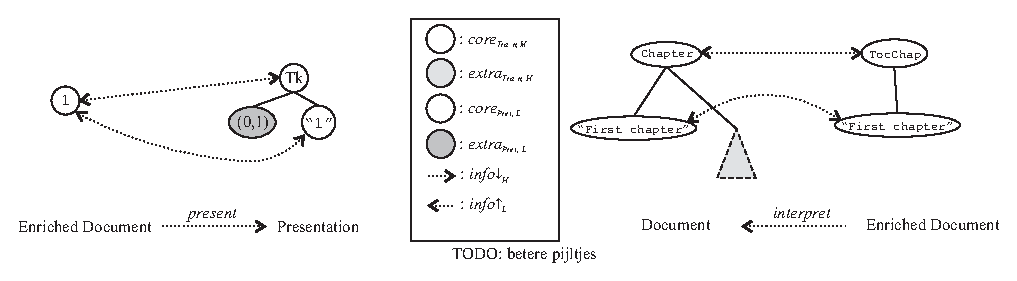
\epsfig{file=pics/eps/coreExtraInfoExamples.eps, width=125mm}
\end{center}
\caption{Two extra state examples with explicit mapping information.}\label{coreExtraInfoExamples} 
\end{center}
\end{figure}

Because the mapping information is part of a level, we define the level type to be a product of $\Info$ and 
$\Extra \times \Core$. Except for the top and bottom levels, all levels contain presentation and interpretation information. The top level is never the result of a presentation mapping, and hence has no presentation information ($\Info\iup$), whereas the bottom level has no interpretation information ($\Info\idwn$). The new definition of $\Level_i$ is:

\begin{small}
\refstepcounter{specification} \label{spec:levelMultiFinal}
\begin{align*}% \label{sse}
\end{align*} 
\(\begin{array}{lcll}
\Level_{0} & = & \Core_{\Intr,0} \times \Extra_{\Intr,0} \times \Info\idwn_{0} \\
\Level_{n} & = & \Core_{\Pres,n} \times \Extra_{\Pres,n} \times  \Info\iup_{n}\\
\lefteqn{\forall i:1 \le i \le n-1:}  \\
\Level_{i} & = & \Core_{\Pres,i} \times \Extra_{\Pres,i}  \times \Info\iup_{i} & \text{\{Viewed from upper layer\}}\\  
               & = & \Core_{\Intr,i} \times \Extra_{\Intr,i} \times \Info\idwn_{i} & \text{\{Viewed from lower layer\}}
\end{array}\)\end{small}
\begin{center}(Specification \thespecification: Level types (Multiple layers, Final))\end{center}\vspace{1em}

*** do we have $\Info\idwn_i = \Info\iup_{i+1}$?

Note that for the middle levels, for which two kinds of mapping information exist, each alternative of the definition contains only one kind. This is because the downward mapping information $\Info\idwn_{i}$ cannot be computed by the higher layers presentation mapping, and hence is part of its extra state: $\Extra_{\Pres,i}$. Analogously, viewed from the lower layer, $\Info\iup_{i}$ is part of $\Extra_{\Intr,i}$. Rather than further complicating the definition by splitting the extra state type in a mapping information part and a regular extra state part (e.g.\ $\Extra_{\Pres,i} = \Extra_{\mathit{Regular},\Pres,i} \times \Info\idwn_{i}$), we choose to make explicit only the mapping information relevant for the direction from which the level is viewed.
\ec

\bc
Again, the notation can be simplified by taking a single layer perspective. Note that we leave the arrows in the  mapping information types, even though they are redundant now.

\begin{small}
\refstepcounter{specification} \label{spec:levelSingleFinal}
\(\begin{array}{lcll} \label{spec:extraStateSL}
\Level_{H} & = & \Core_{H} \times \Extra_{H} \times \Info\idwn_{H}\\
\Level_{L} & = & \Core_{L} \times \Extra_{L} \times \Info\iup_{L}\\
\end{array}\)\end{small}
\begin{center}(Specification \thespecification: Level types (Single layer, Final))\end{center}\vspace{1em}
\ec

\bc
% example in picture 
Figure~\ref{mappingInfo} shows two examples of the $\Info$ argument. The left-hand side shows the situation at the presentation layer of a Haskell source editor during presentation.  The enriched document node \verb|If|  was presented on the three tokens in the presentation level. The downward arrows represent $\Info_{\Pres,H}$, whereas the upward arrows are the interpretation information $\Info_{\Intr, L}$. The dotted arrows represent $\Info_{\Intr,H}$ (upward) and $\Info_{\Pres,L}$ (downward), which are not used in this layer. The whitespace nodes in the presentation level are presentation extra state, that has to be reused on presentation. 
%\note{more detail on reuse?}

The right-hand side of the figure shows the evaluation layer of a word processor during interpretation. The document is a \verb|Chapter| node containing two \verb|Section| children, which is mapped onto a table of contents structure in the evaluation level. Again, downward arrows are $\Info_{\Pres,H}$ and upward arrows are $\Info_{\Intr,L}$. 
%\note{mention there is no $\Info_{\Intr,H}$?} In this case, the document contains interpretation extra state, since the contents of the chapter and sections cannot be computed from the enriched document.  \note{more detail on reuse?}

\begin{figure}
\begin{center}
\begin{center}
\begin{footnotesize}
\begin{verbatim}
Enriched Document:                       Document:                                                                                            
                                                                                            
                  If                         Chapter "chapter 1" {"this is bla bla bla..."} 
            / /   | |   \\                      v       v                                     
           v v    v v    vv              Sect "1" {"..."}     Sect "2" {"..."}                
       ^           ^           ^           |   /                    \   |                            
      /    ^       |   ^        \  ^       v  v          ^  ^        v  v                          
    Token /      Token |      Token \                    |  |                             
 {WS} "if"    {WS} "then"  {WS} "else"      ChapterTocEntry "chapter 1"                     
                                          ^              ^                 ^   ^              
Presentation:                            SectionTocEntry "1"  SectionTocEntry "2"           
                                                                                            
                                         Enriched Document:                                 

----------                                                                        
legend   ^ is pres info       v is intr info     {node} is extra state            
                                                                                  
\end{verbatim}  
\end{footnotesize}                                                                  
\end{center}                                                                      
\caption{Mapping information.}\label{info}                          
\end{center}                                                                      
\end{figure}

%??? 
%Mapping is to the node for reusing. Mapping to path is for associating doc edits with presentation parts.
%If things are moved, the paths are no longer meaningful (nodes are). Before doc op, always fix paths by parsing.


%What about keeping list [ID->Info?] that switches and is not part of level.
We choose to make the mapping information part of the $\Level$ type. The reason for this is that both adjacent layers may update a level, and therefore also affect the mapping information on the level. 
%\note{need an example? ** Johan: ja **} With the mapping information in the level types, $\present$ and $\interpret$ do not need additional arguments anymore.
\ec


